\begin{frame}{$d(K^-, n)"K^0 n"$スペクトラム}
  \tminipageTwo{
    \begin{figure}
      補正前(生カウント)
      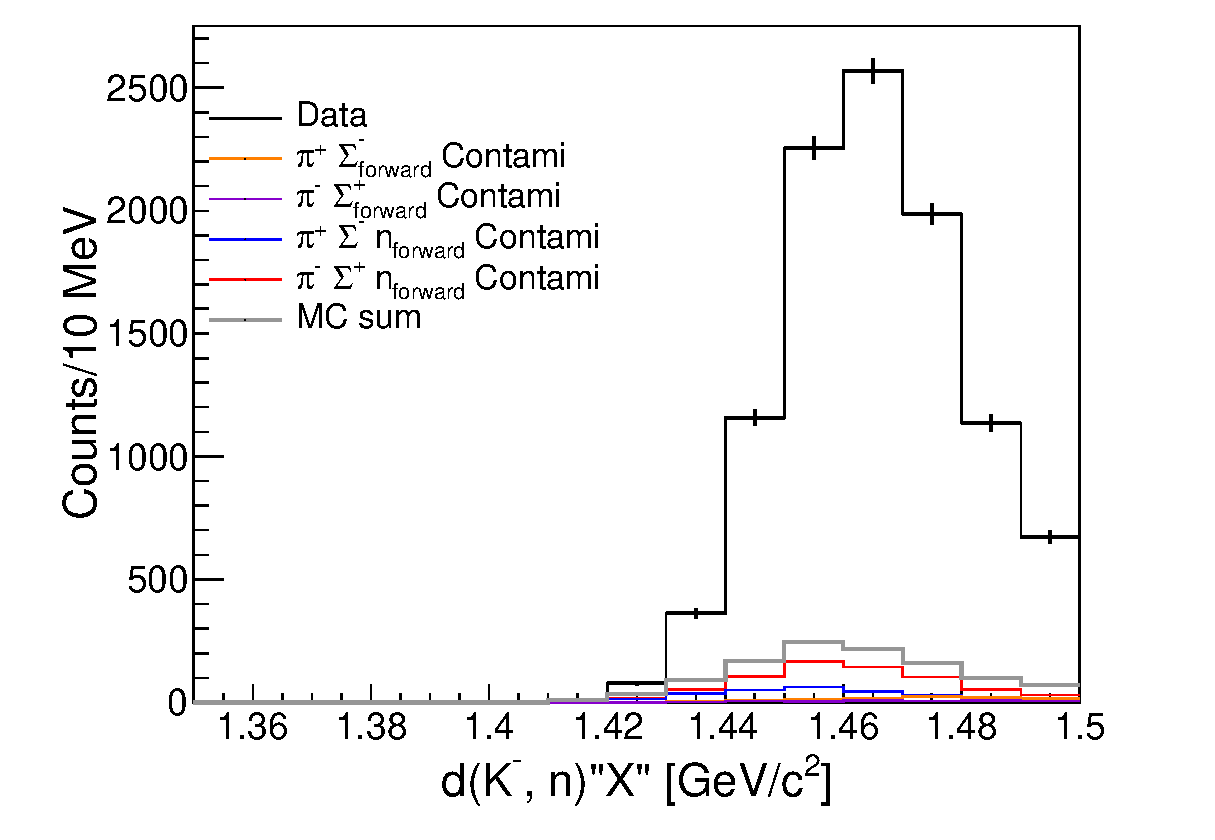
\includegraphics[width=6cm]{../pic/Run78/QE/KN_MM_wK0_tag.eps}
    \end{figure}
  }{
    \begin{figure}
      アクセプタンス補正後
      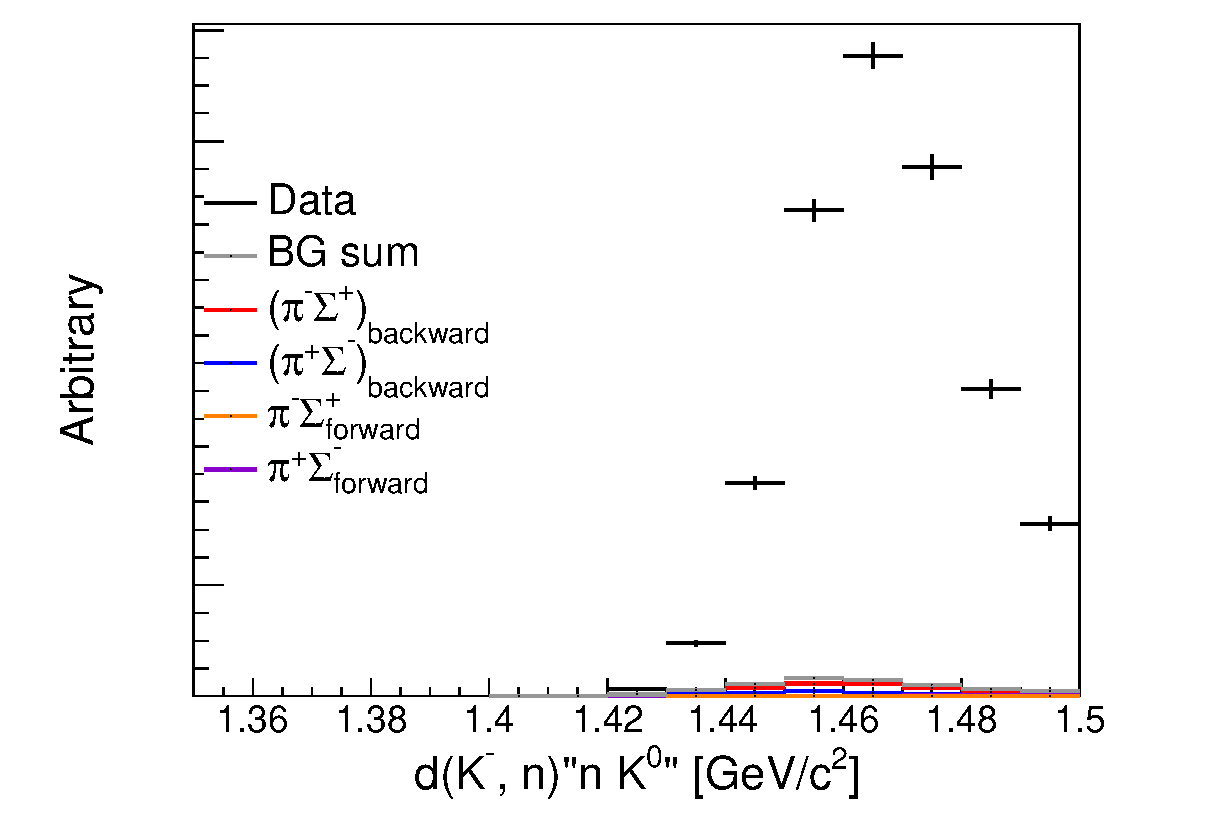
\includegraphics[width=6cm]{../pic/Run78/QE/K0_spec_wBG.eps}
    \end{figure}
  }

  \centering
  データはアクセプタンスの端の低い場所に集中しているので\\
  アクセプタンス補正をするとシグナルが強調されれる。
\end{frame}
